\documentclass[13pt]{beamer}
\usepackage{geometry} %Page setting
\usepackage{hyperref}
\usepackage{amsfonts}
\usepackage{amsmath}
\usepackage{amssymb}
%\usepackage{ctex}
\usepackage{mathtools}
\usepackage{graphicx}
\usepackage{color}
\usetheme{Warsaw}
%\usetheme[height=7mm]{Rochester}

\begin{document}
% Author,title,date,etc.

\title{Projection method for Maxwell equation\\(Mixed finite element method)}
\author{\color{blue}Jiang Guo}
\institute{Nankai University,China\\[1ex]
 E-mail:\texttt{\color{blue}jiangliuer0705@gmail.com}}
\date{March 22,2013}

% The main documents
\begin{frame}
  \titlepage
\end{frame}

\begin{frame}{Outline}
  \tableofcontents
\end{frame}

\section{Projection finite element method for Maxwell equation}

\subsection{curl-curl problem}

\begin{frame}[t]{curl-curl problem}
  \begin{block}{Equation}
   Let $\Omega\subset\mathbb{R}^d (d=2,3)$ be an open,bounded domain with boundary $\Gamma=\partial\Omega.$
We consider the following Maxwell curl-curl problem:
  \begin{eqnarray}
     \triangledown\times\triangledown\times \textbf{u} - \omega^2\mathbf{u} & = & \mathbf{f}, \qquad  in\ \Omega \\
     \triangledown\cdot\mathbf{u}  & = & g, \qquad in \ \Omega \\
     \mathbf{u}\times\mathbf{n} & = & \mathbf{0}, \qquad in\ \Gamma
  \end{eqnarray}
  \end{block}
  \begin{block}{Hilbert Space}
    \begin{equation}\label{space:U_h}
        \nonumber
        {\color{blue}H_0(\triangledown\times;\Omega) = \big\{\mathbf{v}\in (L^2(\Omega))^d : \triangledown\times\mathbf{v}\in (L^2(\Omega))^{2d-3}, \mathbf{v}\times\mathbf{n} = 0\big\}}
        \end{equation}
        \begin{equation}\label{space:U+_h}
        \nonumber
        {\color{blue}\mathcal{U} = (H^1(\Omega))^d\cap H_0(\triangledown\times;\Omega)\cap H(\triangledown\cdot;\Omega)}
    \end{equation}
  \end{block}
\end{frame}

\begin{frame}[t]{curl-curl problem}
  \begin{block}{Classical Variational Form}
    Find $\mathbf{u}\in\mathcal{U}$ such that
    \[(\triangledown\times\mathbf{u},\triangledown\times\mathbf{v}) + (\triangledown\cdot\mathbf{u},\triangledown\cdot\mathbf{v}) - \
    \omega^2(\mathbf{u},\mathbf{v}) = (\mathbf{f},\mathbf{v}) + (g,\triangledown\cdot\mathbf{v}), \qquad \forall\ \mathbf{v}\in\mathcal{U}\]
  \end{block}
  \begin{block}{Definition of Projection}
    \[{\color{blue}Q_h = \{g\in H_{0}^{1}(\Omega): q|_T\in P_1(T), \forall T\in \mathcal{T}_h\}}\]
    \[{\color{blue}W_h = \{w\in (H^{1}(\Omega)\cap L^{2}_{0}(\Omega))^{2d-3}: w|_T\in (P_1(T))^{2d-3}, \forall T\in \mathcal{T}_h\}}\]\\[-5ex]
    \begin{eqnarray}
       && \left\{\begin{array}{cc}
        (\breve{R}_h(\triangledown\cdot\mathbf{v}),q)_{0,h} = - (\mathbf{v},\triangledown q), & \forall q\in Q_h \\
        \breve{R}_h(\triangledown\cdot\mathbf{v})\in Q_h
        \end{array}\right.\\
       && \left\{\begin{array}{cc}
        (R_h(\triangledown\times\mathbf{v}),w)_{0,h} = (\mathbf{v},\triangledown\times w), & \forall w\in W_h \\
        R_h(\triangledown\times\mathbf{v})\in W_h
        \end{array}\right.
    \end{eqnarray}
  \end{block}
\end{frame}

\begin{frame}[t]{curl-curl problem}
   \begin{block}{Projection FEM Variational Form}

     $\quad$Find $\mathbf{u}_h\in\mathcal{U}_h$, such that
     \begin{equation}{\color{red}B_h(\mathbf{u}_h,\mathbf{v}_h) = L_h(\mathbf{v}_h), \forall\ \mathbf{v}_h\in\mathcal{U}_h}\end{equation}
     where
     \[{\color{blue}\mathcal{U}_h = \big\{\mathbf{v}\in \mathcal{U}: \mathbf{v}|_T\in\big(P_{1}^{+}(T)\big)^d, \forall T\in \mathcal{T}_h\big\}} (Mini\ element)\]
     \begin{eqnarray}
         \nonumber
         &&B_h(\mathbf{u}_h,\mathbf{v}_h) := \big(R_h(\triangledown\times\mathbf{u}_h),R_h(\triangledown\times\mathbf{v}_h)\big) \\ \nonumber
         &&\qquad\qquad\qquad + \big(\breve{R}_h(\triangledown\cdot\mathbf{u}_h),\breve{R}_h(\triangledown\cdot\mathbf{v}_h)\big) - \
         \omega^2(\mathbf{u}_h,\mathbf{v}_h)  \\ \nonumber
         &&L_h(\mathbf{v}_h) := (\mathbf{f},\mathbf{v}_h) + \big(g,\breve{R}_h(\triangledown\cdot\mathbf{v}_h)\big) \\ \nonumber
     \end{eqnarray}
   \end{block}

\end{frame}

\begin{frame}[t]{curl-curl problem}
  \begin{block}{Implementation of Projection by Mixed FEM}
    $\quad$Let $\mathcal{M}_h = \mathcal{U}_h\times Q_h\times W_h$, find $(\mathbf{u}_h,p_h,\xi_h)\in\mathcal{M}_h$ such that $\forall(\mathbf{v}_h,q_h,w_h)\in\mathcal{M}_h$, we have the following equations
    \qquad\begin{enumerate}
      \item $(p_h,q_h)_{0,h} + (\mathbf{u}_h,\triangledown q_h) = 0$
      \item $(\xi_h,w_h)_{0,h} - (\mathbf{u}_h,\triangledown\times w) = 0$
      \item $(\triangledown\times p_h,\mathbf{v}_h) - (\triangledown \xi_h,\mathbf{v}_h) -\omega^2(\mathbf{u}_h,\mathbf{v}_h) = ( \mathbf{f},\mathbf{v}_h) + (Sg,\triangledown\cdot\mathbf{v}_h) $
    \end{enumerate}
  where \\
  \qquad$Sg$ is the projection of $g$ onto the space of $Q_h$, namely, find $Sg\in Q_h$ such that \\[-2ex]
  \[(Sg,q_h)_{0,h} = (g,q_h),\quad \forall q_h\in Q_h\]
  Note1: To simplify, we sometimes omit $(.,.)_{0,h}.$
  \end{block}
\end{frame}

\subsection{curl-curl-grad-div problem}
\begin{frame}[t]{curl-curl-grad-div problem}
  \begin{block}{Equation}
   Let $\Omega\subset\mathbb{R}^d (d=2,3)$ be an open,bounded domain with boundary $\Gamma=\partial\Omega.$
We consider the following Maxwell curl-curl-grad-div problem:
  \begin{eqnarray}
     \triangledown\times\triangledown\times \textbf{u} - \triangledown\triangledown\cdot\mathbf{u} - \omega^2\mathbf{u} & = & \mathbf{f}, \qquad  in\ \Omega \\
     \triangledown\times\mathbf{n} & = & \mathbf{0}, \qquad in\ \Gamma\\
     \triangledown\cdot\mathbf{u}  & = & 0, \qquad in \ \Gamma
  \end{eqnarray}
  \end{block}
  \begin{block}{Classical Variational Form}
    Find $\mathbf{u}\in{\color{blue}\mathcal{U}\cap H_0(\triangledown\cdot;\Omega):= \mathcal{U}^{0}}$ such that
    \[(\triangledown\times\mathbf{u},\triangledown\times\mathbf{v}) + (\triangledown\cdot\mathbf{u},\triangledown\cdot\mathbf{v}) - \
    \omega^2(\mathbf{u},\mathbf{v}) = (\mathbf{f},\mathbf{v}), \qquad \forall\ \mathbf{v}\in\mathcal{U}^{0}\]
  \end{block}
\end{frame}

\begin{frame}[t]{curl-curl-grad-div problem}
   \begin{block}{Projection FEM Variational Form}
     $\qquad$Find $\mathbf{u}_h\in\mathcal{U}^{0}_{h}$, such that {\color{red}\[B_h(\mathbf{u}_h,\mathbf{v}_h) = L_h(\mathbf{v}_h), \forall\ \mathbf{v}_h\in\mathcal{U}^{0}_{h}\] }
     where
     \begin{eqnarray}
         \nonumber
         &&{\color{blue}\mathcal{U}_h^0 = \big\{\mathbf{v}\in \mathcal{U}^0: \mathbf{v}|_T\in\big(P_{1}^{+}(T)\big)^d, \forall T\in \mathcal{T}_h\big\}} \\ \nonumber
         &&B_h(\mathbf{u}_h,\mathbf{v}_h) := \big(R_h(\triangledown\times\mathbf{u}_h),R_h(\triangledown\times\mathbf{v}_h)\big) \\ \nonumber
         &&\qquad\qquad\qquad + \big(\breve{R}_h(\triangledown\cdot\mathbf{u}_h),\breve{R}_h(\triangledown\cdot\mathbf{v}_h)\big) - \
         \omega^2(\mathbf{u}_h,\mathbf{v}_h)  \\ \nonumber
         &&L_h(\mathbf{v}_h) := (\mathbf{f},\mathbf{v}_h)
     \end{eqnarray}
     Note2: The implementation of projection by mixed finite element method is similar as curl-curl problem.
   \end{block}
\end{frame}

\section{Projection finite element method for Maxwell eigenproblem}

\subsection{Maxwell Eigenproblem}
\begin{frame}[t]{Maxwell Eigenproblem}
  \begin{block}{}
     \begin{enumerate}
     \item curlcurl eigenproblem

       Find $(\omega^2, \mathbf{u}\neq\mathbf{0})\in\mathbb{R}\times\mathcal{U}^0$, such that
       \begin{equation}
         \nonumber
         \left\{\begin{array}{cc}
           \triangledown\times\mu^{-1}\triangledown\times\mathbf{u} = \omega^2\epsilon\mathbf{u} &  in\ \Omega \\
           \triangledown\cdot\epsilon\mathbf{u} = 0  & on\ \Gamma  \\
           \mathbf{u}\times\mathbf{n} = \mathbf{0}  & on\ \Gamma
         \end{array}\right.
       \end{equation}
     \item curlcurlgraddiv eigenproblem

       Find $(\omega^2, \mathbf{u}\neq\mathbf{0})\in\mathbb{R}\times\mathcal{U}^0$, such that
       \begin{equation}
         \nonumber
         \left\{\begin{array}{cc}
           \triangledown\times\mu^{-1}\triangledown\times\mathbf{u} - \epsilon\triangledown\triangledown\cdot\epsilon\mathbf{u}= \omega^2\epsilon\mathbf{u} &  in\ \Omega \\
           \triangledown\cdot\epsilon\mathbf{u} = 0  & on\ \Gamma  \\
           \mathbf{u}\times\mathbf{n} = \mathbf{0}  & on\ \Gamma
         \end{array}\right.
       \end{equation}
     \end{enumerate}
     Note3: we only consider ccgd eigenproblem, cc is the same.
  \end{block}

\end{frame}

\begin{frame}[t]{Maxwell Eigenproblem}
   \begin{block}{The Classical Variational Form(ccgd)}
    Find $(\omega^2, \mathbf{u}\neq\mathbf{0})\in\mathbb{R}\times\mathcal{U}^0_{\epsilon}$, such that
   {\color{red}
    \[(\mu^{-1}\triangledown\times\mathbf{u},\triangledown\times\mathbf{v}) + \
    s(\triangledown\cdot\epsilon\mathbf{u},\triangledown\cdot\epsilon\mathbf{v}) = \
    \omega^2(\epsilon\mathbf{u},\mathbf{v}),\quad \forall\ \mathbf{v}\in\mathcal{U}^0_{\epsilon}\]
   }
   where

   {\color{blue}
   $\qquad\qquad\mathcal{U}^0_{\epsilon} = H_0(\triangledown\times; \Omega)\cap H_0(\triangledown\cdot \epsilon; \Omega)$
   }\\
   $\qquad s$ is used to distinguish between true and false eigenvalue.\\

   Both sides plus $(\epsilon\mathbf{u},\mathbf{v})$, we have the following equivalent variational form:
   Find $(\lambda, \mathbf{u}\neq\mathbf{0})\in\mathbb{R}\times\mathcal{U}^0_{\epsilon}$ ($\lambda = 1+ \omega^2$), such that
   {\color{red}
    \[(\mu^{-1}\triangledown\times\mathbf{u},\triangledown\times\mathbf{v}) + \
    s(\triangledown\cdot\epsilon\mathbf{u},\triangledown\cdot\epsilon\mathbf{v}) + (\epsilon\mathbf{u},\mathbf{v}) = \
    \lambda(\epsilon\mathbf{u},\mathbf{v}),\quad \forall\ \mathbf{v}\in\mathcal{U}^0_{\epsilon}\]
   }
   \end{block}
\end{frame}

\subsection{Projection Finite Element Method for Maxwell Eigenproblem}
\begin{frame}[t]{Projection FEM for Maxwell Eigenproblem}
  \begin{block}{}
  For any given $\mathbf{v}\in\big(L^2(\Omega)\big)^d$, define $\breve{R}_h(\triangledown\cdot\epsilon\mathbf{v})\in Q_h$ and
  $R_h(\mu^{-1}\triangledown\times\mathbf{v})\in W_h$ as follows:\\[-3ex]
  \begin{eqnarray}
       \nonumber
       (\breve{R}_h(\triangledown\cdot\epsilon\mathbf{v}),q) & = & - (\mathbf{v},\epsilon\triangledown q),\quad  \forall q\in Q_h \\
       \nonumber
       (R_h(\mu^{-1}\triangledown\times\mathbf{v}),w)_{\mu} & = & (\mathbf{v},\triangledown\times w),\quad  \forall w\in W_h
  \end{eqnarray}
  Projection FEM:\\
  $\quad$Find $(\lambda_h, \mathbf{u}_h\neq\mathbf{0})\in\mathbb{R}\times\mathcal{U}^0_{\epsilon h}$ such that\\[-2ex] \[{\color{red}B_h(\mathbf{u_h},\mathbf{v}_h) = \
  \lambda_h(\epsilon\mathbf{u}_h,\mathbf{v}_h),\ \forall\ \mathbf{v_h}\in\mathcal{U}^0_{\epsilon h}}\]
  where: ${\color{blue}\mathcal{U}^0_{\epsilon h} = \big\{\mathbf{v}\in \mathcal{U}^0_{\epsilon}: \mathbf{v}|_T\in\big(P_{1}^{+}(T)\big)^d, \forall T\in \mathcal{T}_h\big\}}$

  $\quad B_h(\mathbf{u_h},\mathbf{v}_h) := \Big(R_h(\mu^{-1}\triangledown\times\mathbf{u}_h),R_h(\mu^{-1}\triangledown\times\mathbf{v}_h)\Big)_{\mu}$ \\ $\qquad\qquad\qquad\quad + s\Big(\breve{R}_h(\triangledown\cdot\epsilon\mathbf{u}_h),\breve{R}_h(\triangledown\cdot\epsilon\mathbf{v}_h)\Big) + \
  (\epsilon\mathbf{u}_h,\mathbf{v}_h)$
  \end{block}
\end{frame}

\section{Numerical results}

\subsection{Example}

\begin{frame}[t]{Example}
   \begin{block}{L-shaped Domain (cc - projection - mixed fem)}
     L-shape domain: $\Omega = [-1,1]^2/[0,1]\times[-1,0]$
     Let $\omega = 1$ and $\varphi(x,y) = r^{\frac{2}{3}}\sin(\frac{2}{3}\theta)$, the exact solution is given by\\[-2ex]
     \[\mathbf{u}(x,y) = \triangledown\big((x^2 - 1)(y^2 - 1)\varphi(x,y)\big)\]
     where $x = r\cos(\theta)$, $y = r\sin(\theta)$ and $(r,\theta)$ is  polar coordinates. \\[-1ex]
     \begin{figure}[bhpt]
         \hspace{-1.pt}
         \begin{minipage}[b]{0.5 \textwidth}
          \centering
          \includegraphics[width=1in]{Image/L-shape}\\
          \caption{L-shape domain}\label{fig:L-shape}
        \end{minipage}
        \hspace{-1.in}
        \begin{minipage}[b]{0.5 \textwidth}
          \centering
          \includegraphics[width=1in]{Image/mesh}\\
          \caption{Mesh}\label{fig:mesh}
        \end{minipage}
     \end{figure}
   \end{block}
\end{frame}

\begin{frame}[t]{Example}
   \begin{block}{Cracked Square Domain (cc - projection - mixed fem)}
     Cracked square domain: $\Omega = [-1,1]^2/[0,1]\times[0]$
     Let $\omega = 1$ and $\varphi(x,y) = r^{\frac{1}{2}}\sin(\frac{1}{2}\theta)$, the exact solution is given by\\[-2ex]
     \[\mathbf{u}(x,y) = \triangledown\big((x^2 - 1)(y^2 - 1)\varphi(x,y)\big)\]
     where $x = r\cos(\theta)$, $y = r\sin(\theta)$ and $(r,\theta)$ is  polar coordinates. \\[-1ex]
     \begin{figure}[bhpt]
         \hspace{-1.pt}
         \begin{minipage}[b]{0.5 \textwidth}
          \centering
          \includegraphics[width=1in]{Image/Crack-square}\\
          \caption{Cracked square domain}\label{fig:L-shape}
        \end{minipage}
        \hspace{-0.6in}
        \begin{minipage}[b]{0.5 \textwidth}
          \centering
          \includegraphics[width=1in]{Image/mesh2}\\
          \caption{Mesh}\label{fig:mesh2}
        \end{minipage}
     \end{figure}
   \end{block}
\end{frame}

\subsection{Numerical Results}
\begin{frame}[shrink=10]{Results}
   \begin{block}{L-shape}
   \begin{center}

   {\color{red} L-shape Relative error of $\mathbf{u}$ by projection-mixed-fem}\\[2ex]
   \begin{tabular}{cccccc}
     \hline
     % after \\: \hline or \cline{col1-col2} \cline{col3-col4} ...
     mesh & 1/4 & 1/8 & 1/16 & 1/32 & 1/64 \\
     \hline
     $\frac{\|u_1 - u_{1h}\|_0}{\|u_1\|_0}$ & 0.08746 & 0.04818 & 0.02870 & 0.01767 & 0.01103 \\
     ratio &  & 1.81 & 1.68 & 1.62 & 1.60  \\
     $\frac{\|u_2 - u_{2h}\|_0}{\|u_2\|_0}$ & 0.13403 & 0.07837 & 0.04795 & 0.02987 & 0.01874 \\
     ratio &  & 1.71 & 1.63 & 1.61 & 1.59  \\
     \hline
   \end{tabular}\\[2ex]
   {\color{red} L-shape Relative error of $\mathbf{u}$ by projection-fem(ssyang)}\\[2ex]
      \begin{tabular}{cccccc}
     \hline
     % after \\: \hline or \cline{col1-col2} \cline{col3-col4} ...
     mesh & 1/4 & 1/8 & 1/16 & 1/32 & 1/64 \\
     \hline
     $\frac{\|u_1 - u_{1h}\|_0}{\|u_1\|_0}$ &0.1903& 0.1115& 0.0684 &0.0427 &0.0268 \\
     ratio &  &1.7067  &1.6301  &1.6019  &1.5933   \\
     $\frac{\|u_2 - u_{2h}\|_0}{\|u_2\|_0}$ &0.1903& 0.1115& 0.0684 &0.0427 &0.0268 \\
     ratio &  &1.7067  &1.6301  &1.6019  &1.5933  \\
     \hline
   \end{tabular}
   \end{center}
   \end{block}
\end{frame}

\begin{frame}[shrink=5]{Results}
  \begin{block}{L-shape}
   \begin{center}
     \includegraphics[width=0.4\textwidth]{Image/L-shape/u1_32.png}
     \includegraphics[width=0.4\textwidth]{Image/L-shape/u1_e_32.png}
   \end{center}
   \begin{center}
     \includegraphics[width=0.4\textwidth]{Image/L-shape/u1_64.png}
     \includegraphics[width=0.4\textwidth]{Image/L-shape/u1_e_64.png}
   \end{center}
  \end{block}
\end{frame}

\begin{frame}[shrink=5]{Results}
  \begin{block}{L-shape}
   \begin{center}
     \includegraphics[width=0.4\textwidth]{Image/L-shape/u2_32.png}
     \includegraphics[width=0.4\textwidth]{Image/L-shape/u2_e_32.png}
   \end{center}
   \begin{center}
     \includegraphics[width=0.4\textwidth]{Image/L-shape/u2_64.png}
     \includegraphics[width=0.4\textwidth]{Image/L-shape/u2_e_64.png}
   \end{center}
  \end{block}
\end{frame}

\begin{frame}[shrink=5]{Results}
  \begin{block}{L-shape}
     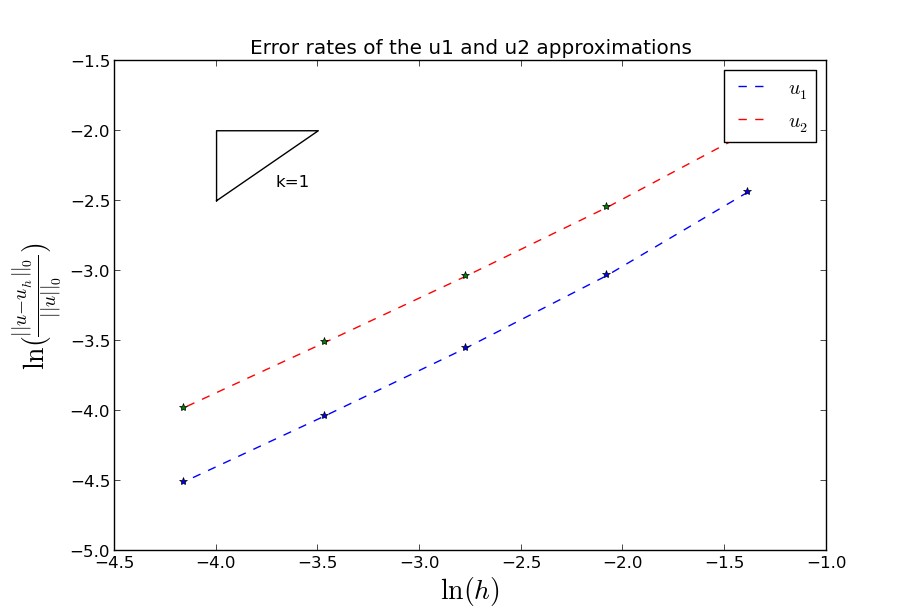
\includegraphics[width=1.0\textwidth]{Image/L-shape_rate.png}
  \end{block}
\end{frame}

%\begin{frame}[shrink=10]{Results}
%   \begin{block}{Cracked-square}
%   \begin{center}
%     \  \ \\[18ex]
%     {\color{red}Sorry, I don't have the right result! }\\
%     \  \ \\[18ex] \  \
%   \end{center}
%   \end{block}
%\end{frame}


\begin{frame}[shrink=10]{Results}
   \begin{block}{Cracked-square}
   \begin{center}

   {\color{red} Cracked-square Relative error of $\mathbf{u}$ by projection-mixed-fem}\\[2ex]
   \begin{tabular}{cccccc}
     \hline
     % after \\: \hline or \cline{col1-col2} \cline{col3-col4} ...
     mesh & 1/8 & 1/16 & 1/32 & 1/64 & 1/128\\
     \hline
     $\frac{\|u_1 - u_{1h}\|_0}{\|u_1\|_0}$ &
     4.32192 & 1.73049 & 0.79694 & 0.39595 &
     0.206631 \\
     ratio &  & 2.45 & 2.17 & 2.01 & 1.92  \\
     $\frac{\|u_2 - u_{2h}\|_0}{\|u_2\|_0}$ & 4.3627 & 1.7712 & 0.83032 & 0.423606 & 0.230516 \\
     ratio &  & 2.46 & 2.13 & 1.96 & 1.83  \\
     \hline
   \end{tabular}\\[2ex]

   \end{center}
   \end{block}
\end{frame}


\begin{frame}[shrink=5]{Results}
  \begin{block}{Cracked-square}
   \begin{center}
     \includegraphics[width=0.4\textwidth]{Image/Cracked-square/u1_64.png}
     \includegraphics[width=0.4\textwidth]{Image/Cracked-square/u1_e_64.png}
   \end{center}
   \begin{center}
     \includegraphics[width=0.4\textwidth]{Image/Cracked-square/u1_128.png}
     \includegraphics[width=0.4\textwidth]{Image/Cracked-square/u1_e_128.png}
   \end{center}
  \end{block}
\end{frame}

\begin{frame}[shrink=5]{Results}
  \begin{block}{Cracked-square}
  \begin{center}
     \includegraphics[width=0.4\textwidth]{Image/Cracked-square/u2_64.png}
     \includegraphics[width=0.4\textwidth]{Image/Cracked-square/u2_e_64.png}
   \end{center}
   \begin{center}
     \includegraphics[width=0.4\textwidth]{Image/Cracked-square/u2_128.png}
     \includegraphics[width=0.4\textwidth]{Image/Cracked-square/u2_e_128.png}
   \end{center}
  \end{block}
\end{frame}

\begin{frame}[shrink=5]{Results}
  \begin{block}{L-shape}
     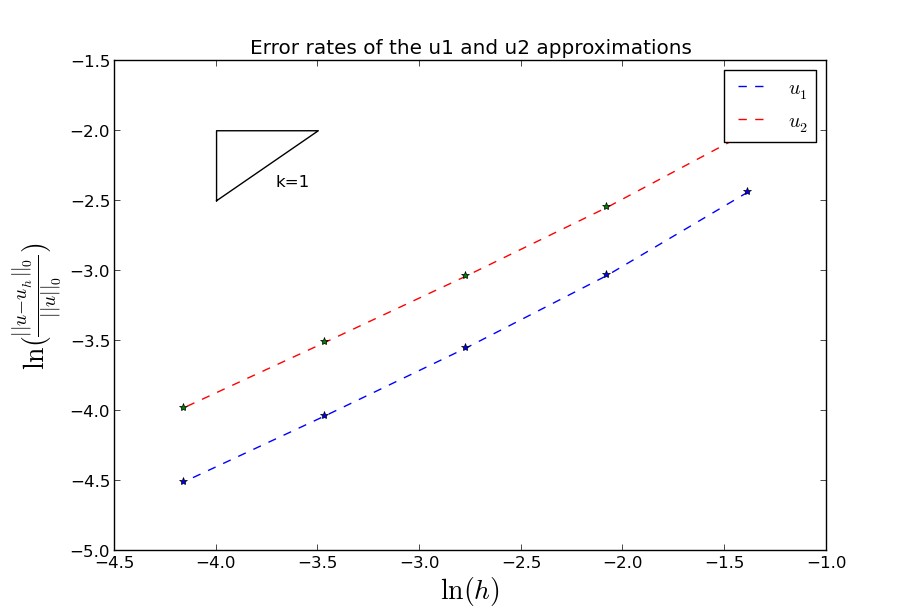
\includegraphics[width=1.0\textwidth]{Image/L-shape_rate.png}
  \end{block}
\end{frame}

%\begin{frame}[t]{Results}
%  \begin{block}{Question}
%     \begin{itemize}
%       \item In L-shape domain, why the error of $u_1\neq$ the error of $u_2$
%       \item The relationship between projection method and mixed-projection method.
%       \item Why the program of cracked-square domain is wrong?
%     \end{itemize}
%  \end{block}
%\end{frame}

\end{document}
